\subsubsection{Skyscarper}
\label{Skyscarper}
Die Technik \textit{Skyscarper} bedeutet übersetzt Wolkenkratzer und leitet sich von der Anordnung der betrachteten Ziffern ab. Gesucht werden zwei Zeilen oder Spalten, in deren Kandidatenlisten die Ziffer jeweils noch genau zwei mal auftaucht. Wenn nun zwei der Kandidaten in der selben anderen Figur (Spalte oder Zeile) sind, dann hat man einen Wolkenkratzer gefunden. Die beiden Zahlen, die in der selben anderen Figur sind, bilden das Fundament des Woleknkratzers, sie schließen sich gegenseitig aus. Das bedeutet wiederum, dass eine der beiden anderen gefundenen Ziffern dort stehen muss. Daher können alle Kandidaten, die von beiden Ziffern ausgeschlossen werden, aus den Kandidatenlisten gelöscht werden.	

\begin{figure}[h]
\begin{center}
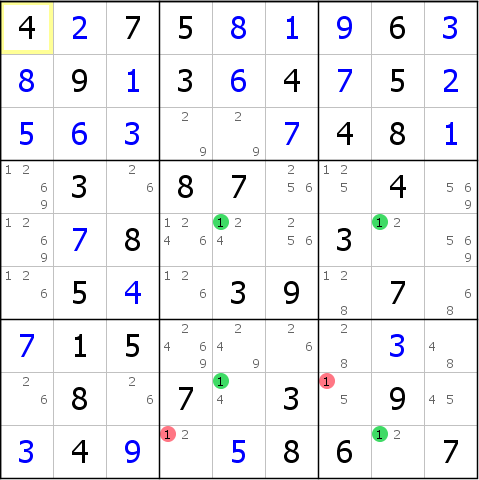
\includegraphics{./img/skyscarper.png}
\caption{Skyscarper}
\end{center}
\end{figure}

In \textbf{Abbildung 3.9} betrachten wir die Spalten 6 und 9. Hier sind die Bedingungen für den Wolkenkratzer erfüllt, da in jeder Spalte die Ziffer 1 jeweils genau zwei mal vorkommt und sie in jeder Spalte an Position 5 auftaucht. Für das Feld z3s9 gibt es nun zwei Möglichkeiten. Entweder die Ziffer 1 steht in diesem Feld oder nicht. Diese beiden Möglichkeiten werden nun separat betrachtet. Wenn die Ziffer 1 in Feld z3s9 steht, dann schließt das bereits alle rot markierten Zahlen aus. Für den Fall, dass die Ziffer 1 nicht in z3s9 steht, muss sie in z5s9 stehen, das geht aus der Bedingung des Wolkenkratzers hervor. Da sich nun z5s9 und z5s6 laut Bedingung in der selben Zeile befinden, kann die Ziffer 1 nicht in z5s6 vorkommen. Deshalb muss sie in z1s6 stehen, wo sie alle rot markierten Felder ausschließt.